\documentclass[11pt, a4paper]{article}

% --- 1. Kodowanie i fonty ---
\usepackage[utf8]{inputenc}
\usepackage[T1]{fontenc}
\usepackage{lmodern}      % Lepszy, wektorowy font
\usepackage{microtype}    % Optymalizacja kerningu i składu tekstu

% --- 2. Ustawienia strony i akapitów ---
\usepackage[margin=1in]{geometry}
\setlength{\parskip}{0.4em}
\setlength{\parindent}{0pt}

% --- 3. Pakiety matematyczne i graficzne ---
\usepackage{amsmath,amssymb}
\usepackage{graphicx}
\usepackage[section]{placeins}

% --- 4. Tabele ---
\usepackage{booktabs}     % Profesjonalne linie (\toprule, \midrule)
\usepackage{array}
\usepackage{multirow}
\usepackage{tabularx}
\usepackage{longtable}

\newcolumntype{L}[1]{>{\raggedright\arraybackslash}p{#1}}
\newcolumntype{C}[1]{>{\centering\arraybackslash}p{#1}}

\newcommand{\stdtablefont}{\small}
\newcommand{\stdtablelayout}{%
  \stdtablefont
  \setlength{\tabcolsep}{4pt}
  \renewcommand{\arraystretch}{1.2}
}

% --- 5. Linki i Spis Treści (Fix dla numerów S10+) ---
\usepackage[colorlinks=true, linkcolor=blue, citecolor=blue, urlcolor=blue]{hyperref}
\usepackage[titles]{tocloft}
\addtolength{\cftsecnumwidth}{1.5em} % Więcej miejsca na prefix "S" i liczby dwucyfrowe

% --- 6. Numeracja Supplementary ---
\renewcommand{\thetable}{S\arabic{table}}
\renewcommand{\thefigure}{S\arabic{figure}}
\renewcommand{\thesection}{S\arabic{section}}

% --- 7. Tytuł i Autorzy ---
\title{%
  \vspace{-1.5cm}
  \LARGE \textbf{Supplementary Material} \\[1.5em]
  \normalsize for the manuscript: \\[0.5em]
  \Large \textit{Relative Logistic Regression: A Probabilistic Refinement \\ of Hard-Voting Pair-Based Omics Classification} \\[1.5em]
  \small submitted to \textit{Computer Methods and Programs in Biomedicine}
}

\author{Marcin Czajkowski, Anna Czajkowska, Krzysztof Jurczuk, and Marek Kretowski}
\date{}

\begin{document}

\maketitle


\tableofcontents
\newpage
%%%%%%%%%%%%%%%%%%%%%%%%%%%

\section*{Overview}

This supplementary document provides additional analyses supporting the main manuscript, with emphasis on aspects that are important for interpreting Relative Logistic Regression (RLR): exploratory candidate-pool and rank-margin sensitivity screens, adaptive-$k$ and post-hoc calibration checks for hard-voting baselines, structural and functional inspection in the PTB fixed-split case study, historical positioning under the legacy eight-dataset benchmark, reliability-oriented score diagnostics, and approximate runtime characterization.

The supplementary analyses are restricted to configurations directly relevant to the final paper. The document focuses on the finalized strict gene-disjoint RLR formulation used in the main manuscript; technical overlap-control configurations are treated only as implementation or multiplicity context where necessary.

\section{Evaluation settings and analytical roles}

Table~\ref{tab:setting_roles} summarizes the analytical role of each evaluation setting used in the study.

\begin{table}[!htbp]
\centering
\caption{Analytical roles of the evaluation settings used in the study.}
\label{tab:setting_roles}
{\stdtablelayout
\begin{tabularx}{\textwidth}{L{0.19\textwidth}L{0.21\textwidth}L{0.23\textwidth}L{0.23\textwidth}}
\toprule
\textbf{Setting} & \textbf{Protocol} & \textbf{Role in the manuscript} & \textbf{Primary interpretation} \\
\midrule
\emph{CompCancer} & Repeated cross-validation across 11 datasets & Primary comparative benchmark & Main inferential setting for model comparison and statistical testing \\
\emph{PTB fixed-split} & Predefined 103/44 split of pooled discovery data & Structural case study & Inspection of fitted pair-based structure, coefficient allocation, and local activity \\
\emph{PTB LOCO} & Leave-one-cohort-out over four cohorts & Cross-cohort stress test & Descriptive evaluation under stronger cohort heterogeneity \\
\emph{legacy8} & Repeated 5-fold cross-validation with 10 repetitions & Historical benchmark & Historical positioning under a classical microarray protocol \\
\bottomrule
\end{tabularx}
}
\end{table}

\section{Dataset inventory for the primary CompCancer benchmark}

The primary \emph{CompCancer} benchmark comprised 11 independent binary transcriptomic datasets:
\emph{alizadeh-2000-v1},
\emph{armstrong-2002-v1},
\emph{bittner-2000},
\emph{chen-2002},
\emph{golub-1999-v1},
\emph{gordon-2002},
\emph{pomeroy-2002-v1},
\emph{shipp-2002-v1},
\emph{singh-2002},
\emph{west-2001}, and
\emph{yeoh-2002-v1}.

These datasets served as the primary inferential basis of the study. In the finalized benchmark protocol, nine datasets were evaluated with 10 repetitions of stratified 5-fold cross-validation, whereas \emph{west-2001} and \emph{yeoh-2002-v1} were evaluated with 2 repetitions, yielding 470 outer test folds per model across the complete benchmark. Results were first aggregated within dataset and then compared across datasets, so that repeated outer folds from the same dataset were not treated as independent inferential units.

\begin{table}[!htbp]
\centering
\caption{Finalized resampling schedule for the 11 \emph{CompCancer} datasets. Each repetition used stratified 5-fold cross-validation.}
\label{tab:compcancer_repetitions}
{\stdtablelayout
\begin{tabular}{lc}
\toprule
\textbf{Dataset} & \textbf{Repetitions} \\
\midrule
alizadeh-2000-v1 & 10 \\
armstrong-2002-v1 & 10 \\
bittner-2000 & 10 \\
chen-2002 & 10 \\
golub-1999-v1 & 10 \\
gordon-2002 & 10 \\
pomeroy-2002-v1 & 10 \\
shipp-2002-v1 & 10 \\
singh-2002 & 10 \\
west-2001 & 2 \\
yeoh-2002-v1 & 2 \\
\bottomrule
\end{tabular}
}
\end{table}

\section{Primary \emph{CompCancer} paired statistical summaries}

Formal inference in the primary benchmark used datasets, rather than individual outer resampling folds, as the paired units. For each model and metric, split-level results were first averaged within dataset. The three paper-focus comparisons were RLR-10 versus $k$-TSP-10, RLR-20 versus $k$-TSP-20, and RLR-50 versus $k$-TSP-50. Paired Wilcoxon signed-rank tests were then applied across the 11 dataset-level values. The configured analysis also contained the technical RLR-50 $d=2$ versus $d=1$ comparison; consequently, Holm adjustment was performed over the complete within-world family of 20 tests (four comparisons across five metrics), while Table~\ref{tab:compcancer_stats} displays only the 15 paper-focus tests.

\begin{table*}[!htbp]
\centering
\caption{Dataset-level paired statistical summaries for the three paper-focus comparisons in the finalized \emph{CompCancer} benchmark. Mean values are averages of the 11 dataset-level summaries. The paired difference is RLR minus $k$-TSP. Holm-adjusted $p$-values come from the complete configured family of 20 within-world tests, including the technical RLR-50 $d=2$ versus $d=1$ comparison not shown here.}
\label{tab:compcancer_stats}
{\scriptsize
\setlength{\tabcolsep}{3pt}
\renewcommand{\arraystretch}{1.15}
\begin{tabular}{llrrrrrr}
\toprule
\textbf{Comparison} & \textbf{Metric} & \textbf{Mean RLR} & \textbf{Mean $k$-TSP} & \textbf{Median diff.} & \textbf{Mean diff.} & \textbf{Raw $p$} & \textbf{Holm $p$} \\
\midrule
RLR-10 vs. $k$-TSP-10 & Logloss & 0.3051 & 0.3782 & -0.0464 & -0.0731 & 0.1000 & 1.0000 \\
 & Brier & 0.0727 & 0.0920 & -0.0122 & -0.0193 & 0.0830 & 1.0000 \\
 & ECE & 0.1055 & 0.1907 & -0.0802 & -0.0852 & 0.0039 & 0.0771 \\
 & AUC & 0.9510 & 0.9556 & 0.0001 & -0.0046 & 0.3983 & 1.0000 \\
 & F1 & 0.8529 & 0.8603 & 0.0057 & -0.0074 & 0.6248 & 1.0000 \\
\midrule
RLR-20 vs. $k$-TSP-20 & Logloss & 0.2672 & 0.3465 & -0.0778 & -0.0793 & 0.1197 & 1.0000 \\
 & Brier & 0.0687 & 0.0959 & -0.0216 & -0.0272 & 0.0185 & 0.2770 \\
 & ECE & 0.0987 & 0.2127 & -0.1084 & -0.1140 & 0.0039 & 0.0771 \\
 & AUC & 0.9552 & 0.9597 & -0.0043 & -0.0045 & 0.2622 & 1.0000 \\
 & F1 & 0.8669 & 0.8717 & 0.0011 & -0.0047 & 1.0000 & 1.0000 \\
\midrule
RLR-50 vs. $k$-TSP-50 & Logloss & 0.2260 & 0.3776 & -0.1400 & -0.1516 & 0.0051 & 0.0816 \\
 & Brier & 0.0633 & 0.1109 & -0.0428 & -0.0476 & 0.0039 & 0.0771 \\
 & ECE & 0.1031 & 0.2435 & -0.1447 & -0.1404 & 0.0039 & 0.0771 \\
 & AUC & 0.9574 & 0.9628 & -0.0031 & -0.0053 & 0.3590 & 1.0000 \\
 & F1 & 0.8686 & 0.8836 & 0.0067 & -0.0150 & 1.0000 & 1.0000 \\
\bottomrule
\end{tabular}
}
\end{table*}

The statistical results reinforce the deliberately narrow interpretation used in the main manuscript. Probability-oriented differences were consistently directed toward lower values for RLR, but after adjustment none of the paper-focus tests crossed the conventional 0.05 threshold. AUC and F1 differences were small and mixed at the dataset level. The primary claim is therefore based on the magnitude and consistency of the score-quality pattern across datasets rather than on statistical significance alone.

\section{Exploratory candidate-pool sensitivity under the disjoint shortlist construction}
The main manuscript uses a strict gene-disjoint RLR shortlist construction together with an upstream candidate pool of 1000 ranked relations. To examine the sensitivity of this design choice without conflating the analysis with the finalized primary resampling schedule, we use a separate exploratory screen in which all 11 \emph{CompCancer} datasets were configured for 10 repetitions of stratified 5-fold cross-validation. The screen used $m=10$, $d=2$, $\alpha=0.5$, \texttt{lambda.min}, and the same deterministic seed as the main pipeline. The pool=10/50 and pool=100 results were obtained in the candidate-pool screen, whereas the pool=1000 reference was taken from the corresponding 10-repetition screening configuration. Consequently, all rows in Table~\ref{tab:pool_ablation} belong to the same exploratory resampling regime and are intentionally kept separate from the frozen primary-benchmark estimates reported in the main manuscript.

\begin{table*}[!htbp]
\centering
\caption{Exploratory candidate-pool sensitivity under the strict gene-disjoint shortlist construction ($m=10$, $d=2$), using 10 repetitions of stratified 5-fold cross-validation for each of the 11 \emph{CompCancer} datasets. These screening-state values are not numerically interchangeable with the frozen primary-benchmark summaries, in which two datasets use only 2 repetitions.}
\label{tab:pool_ablation}
{\stdtablelayout
\begin{tabular}{lcccccccccc}
\toprule
\textbf{Model} & \textbf{$K$} & \textbf{Pool} & \textbf{AUC} & \textbf{F1} & \textbf{Logloss} & \textbf{Brier} & \textbf{ECE} & \textbf{Active} & \textbf{Unique} & \textbf{Local active} \\
 & & & & & & & & \textbf{pairs} & \textbf{genes} & \textbf{mean} \\
\midrule
RLR-10  & 10 & 10   & 0.931 & 0.814 & 0.392 & 0.092 & 0.120 & 3.85  & 7.71  & 3.56 \\
RLR-10  & 10 & 100  & 0.950 & 0.846 & 0.307 & 0.075 & 0.108 & 8.58  & 17.15 & 7.88 \\
RLR-10  & 10 & 1000 & 0.950 & 0.849 & 0.304 & 0.074 & 0.107 & 9.35  & 18.69 & 8.45 \\
\midrule
RLR-20  & 20 & 1000 & 0.956 & 0.867 & 0.264 & 0.067 & 0.098 & 16.69 & 33.38 & 15.14 \\
\midrule
RLR-50  & 50 & 50   & 0.946 & 0.844 & 0.311 & 0.077 & 0.108 & 8.06  & 16.11 & 7.46 \\
RLR-50  & 50 & 100  & 0.953 & 0.850 & 0.285 & 0.072 & 0.103 & 11.23 & 22.46 & 10.37 \\
RLR-50  & 50 & 1000 & 0.958 & 0.867 & 0.227 & 0.062 & 0.103 & 27.97 & 55.94 & 25.44 \\
\bottomrule
\end{tabular}
}
\end{table*}

The exploratory screen indicates that highly restrictive upstream pools can constrain the disjoint shortlist and are accompanied by poorer probability-oriented score summaries. The effect is most evident when the available candidate pool is small relative to the target shortlist size. For the compact configuration, the difference between pool=100 and pool=1000 is small, whereas the larger $K=50$ configuration benefits more clearly from the broader upstream pool. This analysis is descriptive and supports the practical use of a broad candidate pool; it is not used as a second inferential benchmark or as an estimate of the final primary-benchmark performance.

The intermediate $K=20$ configuration is shown only at pool=1000 as a reference between the compact and larger regimes. Because the candidate-pool screen and the frozen primary benchmark use different repetition schedules for \emph{west-2001} and \emph{yeoh-2002-v1}, the screening-state pool=1000 values in Table~\ref{tab:pool_ablation} differ slightly from the final main-text values by design.

%%%%%

\section{Exploratory rank-margin sensitivity screen}

Because the ternary encoding used by RLR depends on the rank-margin parameter $m$, we additionally examined $m\in\{1,5,10,20,50\}$ in an earlier exploratory \emph{CompCancer} screen. This screen used 2 repetitions of stratified 5-fold cross-validation for each of the 11 datasets, with $K\in\{10,20,50\}$, $d=2$, an upstream pool of 1000 relations, $\alpha=0.5$, and \texttt{lambda.min}. It therefore differs from the frozen primary benchmark, in which nine datasets use 10 repetitions and two datasets use 2 repetitions. Consequently, the $m=10$ rows in Table~\ref{tab:m_sensitivity_world} are not duplicate estimates of the final main-text $m=10$ results and should not be compared numerically with them as if they arose from the same resampling schedule.

Across the exploratory screen, middle margin values were broadly stable across all three target shortlist sizes. A very large margin ($m=50$) reduced local active evidence and generally worsened probability-oriented behavior, especially for the larger configurations. The purpose of this analysis is therefore limited: it shows that the qualitative behavior of the ternary encoding is not confined to a single margin value. No dataset-specific margin selection was performed in the finalized benchmark, which used the fixed value $m=10$ throughout.

\begin{table*}[!htbp]
\centering
\caption{Exploratory rank-margin sensitivity screen for \emph{CompCancer}, based on 2 repetitions of stratified 5-fold cross-validation for each of the 11 datasets. These screening-state summaries characterize qualitative dependence on $m$ and are not numerically interchangeable with the frozen primary-benchmark summaries. Middle margin values are broadly similar, whereas a very large margin reduces local active evidence and generally worsens probability-oriented performance.}
\label{tab:m_sensitivity_world}
{\stdtablelayout
\begin{tabular}{cccccc}
\toprule
\textbf{$K$} & \textbf{$m$} & \textbf{Logloss} & \textbf{Brier} & \textbf{ECE} & \textbf{Local active} \\
 & & & & & \textbf{mean} \\
\midrule
10 & 1  & 0.275 & 0.066 & 0.097 & 8.81 \\
10 & 5  & 0.277 & 0.067 & 0.098 & 8.62 \\
10 & 10 & 0.269 & 0.065 & 0.098 & 8.49 \\
10 & 20 & 0.276 & 0.067 & 0.099 & 8.17 \\
10 & 50 & 0.293 & 0.071 & 0.102 & 7.28 \\
\midrule
20 & 1  & 0.250 & 0.064 & 0.094 & 15.71 \\
20 & 5  & 0.249 & 0.063 & 0.092 & 15.38 \\
20 & 10 & 0.247 & 0.063 & 0.091 & 15.16 \\
20 & 20 & 0.259 & 0.064 & 0.094 & 14.57 \\
20 & 50 & 0.268 & 0.068 & 0.100 & 13.01 \\
\midrule
50 & 1  & 0.223 & 0.060 & 0.098 & 26.66 \\
50 & 5  & 0.222 & 0.060 & 0.097 & 25.93 \\
50 & 10 & 0.219 & 0.060 & 0.098 & 25.35 \\
50 & 20 & 0.228 & 0.061 & 0.098 & 24.35 \\
50 & 50 & 0.239 & 0.066 & 0.105 & 21.55 \\
\bottomrule
\end{tabular}
}
\end{table*}

The clearest practical pattern in this exploratory screen is structural as well as predictive. As $m$ increases, the local active footprint decreases monotonically or near-monotonically, reflecting the widening no-signal region of the ternary encoding. Moderate margin values preserve this sparsifying effect without a large change in the screening-state score summaries, whereas a very large margin suppresses more local evidence and is accompanied by worse probability-oriented values. Because this screen is not the frozen primary benchmark, only these qualitative trends are carried forward into the interpretation of the main analysis.


\section{Exploratory adaptive-$k$ hard-voting baseline in the primary benchmark}

A possible concern about the main-text hard-voting baselines is that they use fixed shortlist sizes, whereas a classical $k$-TSP workflow can also be formulated with data-dependent selection of the final number of retained pairs. To probe this issue more directly, we ran an additional exploratory adaptive-$k$ variant of $k$-TSP in the primary \emph{CompCancer} benchmark, using three upper limits ($k_{\max}=10,20,50$). These runs were treated as a supplementary robustness check rather than as part of the main benchmark design.

Table~\ref{tab:adaptive_ktsp_world} shows that the adaptive hard-voting baseline did not emerge as a stronger overall comparator than the fixed-$k$ baselines used in the main manuscript. Even when larger upper limits were allowed, the selected models remained relatively compact: the mean realized shortlist size increased only from 6.6 to 8.8 and then to 11.7 as $k_{\max}$ increased from 10 to 20 and 50. Thus, the adaptive procedure did not typically favor large hard-voting models in this benchmark.

At the predictive level, the adaptive hard-voting models had higher world-level logloss and Brier score than the corresponding main-text RLR configurations. Their logloss ranged from 0.526 to 0.494, whereas the canonical RLR values ranged from 0.305 to 0.226. Expected calibration error was somewhat lower than for the larger fixed-$k$ hard-voting baselines, but the adaptive procedure did not reproduce the probability-oriented score summaries of the complete RLR pipeline.

At the dataset level, the adaptive procedure also remained structurally conservative. Even with $k_{\max}=50$, six of the eleven datasets still had a mean selected shortlist size below 10. This suggests that the main probability-oriented advantage of RLR in \emph{CompCancer} is not simply an artifact of having compared against overly large hard-voting baselines.

\begin{table*}[!htbp]
\centering
\caption{Exploratory adaptive-$k$ hard-voting results in the primary \emph{CompCancer} benchmark. Reported values are world-level summaries across the 11 datasets. The adaptive procedure selected relatively compact models even when larger upper limits were allowed, and did not yield a stronger overall comparator than the fixed-$k$ baselines used in the main manuscript.}
\label{tab:adaptive_ktsp_world}
{\stdtablelayout
\begin{tabular}{lccccccc}
\toprule
\textbf{Model} & \textbf{$k_{\max}$} & \textbf{Selected} & \textbf{AUC} & \textbf{F1} & \textbf{Logloss} & \textbf{Brier} & \textbf{ECE} \\
 & & \textbf{$k$ mean} & & & & & \\
\midrule
Adaptive $k$-TSP & 10 & 6.61  & 0.948 & 0.849 & 0.526 & 0.095 & 0.174 \\
Adaptive $k$-TSP & 20 & 8.81  & 0.952 & 0.856 & 0.495 & 0.095 & 0.180 \\
Adaptive $k$-TSP & 50 & 11.68 & 0.953 & 0.858 & 0.494 & 0.096 & 0.183 \\
\bottomrule
\end{tabular}
}
\end{table*}

Relative to the fixed-$k$ hard-voting baselines in the main manuscript, the adaptive procedure did not yield a stronger overall comparator. At the world level, adaptive $k$-TSP reached AUC values of 0.948/0.952/0.953 and F1 values of 0.849/0.856/0.858 for $k_{\max}=10/20/50$, respectively, while its logloss remained 0.526/0.495/0.494. These values do not materially strengthen the hard-voting baseline relative to the fixed-$k$ comparisons used in the main paper, and they remain clearly weaker than the corresponding main-text RLR configurations in probability-oriented performance, for which logloss was 0.305/0.267/0.226 for RLR-10/20/50. Thus, allowing the hard-voting baseline to choose its own final shortlist size does not alter the main conclusion of the paper: the clearest advantage of RLR remains concentrated in score quality rather than in universal dominance across all predictive metrics.


\section{Post-hoc calibration of vote-derived $k$-TSP scores in the primary benchmark}

Because classical $k$-TSP produces coarse vote-derived scores rather than probabilities from an explicitly fitted probabilistic model, we additionally examined whether part of the probability-quality gap to RLR could be reduced by post-hoc calibration. This analysis was treated as a supplementary fairness check rather than as part of the main benchmark design.

For each outer split of the primary \emph{CompCancer} benchmark, calibration was performed strictly within the outer training data. Specifically, pooled out-of-fold raw vote-fraction scores from the outer training portion were used to fit either a Platt-scaling calibrator or an isotonic calibrator. The $k$-TSP model was then refit on the full outer training set, raw scores were computed on the outer test set, and the previously learned calibration mapping was applied to obtain calibrated probabilities. Raw scores were normalized by the realized number of retained pairs in each split.

Table~\ref{tab:calibrated_ktsp_world} shows that Platt scaling substantially improved the probability-oriented behavior of classical $k$-TSP, especially in logloss, Brier score, and expected calibration error. However, these gains did not eliminate the gap to the corresponding main-text RLR configurations, particularly for the intermediate and higher-capacity settings. By contrast, isotonic calibration was unstable in this benchmark: although expected calibration error was sometimes lower, logloss deteriorated markedly, suggesting that a more flexible monotone remapping was not reliable on these coarse vote-derived score scales.

Thus, the calibrated-$k$-TSP analysis supports a more nuanced interpretation of the main results. Post-hoc remapping improves the probability-oriented behavior of classical vote-derived scores, but it does not reproduce the results of the complete RLR pipeline in the intermediate and larger configurations. Because RLR also differs from classical $k$-TSP in relational encoding, candidate refinement, shortlist construction, and regularized fitting, the residual difference cannot be attributed to any single RLR component from this comparison alone.

\begin{table*}[!htbp]
\centering
\caption{Post-hoc calibration of vote-derived $k$-TSP scores in the primary \emph{CompCancer} benchmark. Calibration was learned strictly within each outer training split using pooled out-of-fold vote-fraction scores. To avoid duplicating the uncalibrated baseline values already reported in the main manuscript, this table focuses only on the calibrated variants. Platt scaling substantially improved probability-oriented metrics relative to the corresponding uncalibrated hard-voting baselines, but did not eliminate the gap to the corresponding main-text RLR configurations. Isotonic calibration was unstable, especially in logloss.}
\label{tab:calibrated_ktsp_world}
{\stdtablelayout
\begin{tabular}{lcccccc}\toprule
\textbf{Model} & \textbf{Calibrator} & \textbf{AUC} & \textbf{F1} & \textbf{Logloss} & \textbf{Brier} & \textbf{ECE} \\
\midrule
$k$-TSP-10 & Platt    & 0.953 & 0.857 & 0.308 & 0.070 & 0.110 \\
$k$-TSP-10 & isotonic & 0.938 & 0.857 & 1.017 & 0.077 & 0.093 \\
\midrule
$k$-TSP-20 & Platt    & 0.956 & 0.872 & 0.333 & 0.065 & 0.104 \\
$k$-TSP-20 & isotonic & 0.943 & 0.869 & 1.056 & 0.071 & 0.090 \\
\midrule
$k$-TSP-50 & Platt    & 0.961 & 0.874 & 0.326 & 0.063 & 0.102 \\
$k$-TSP-50 & isotonic & 0.949 & 0.873 & 0.912 & 0.067 & 0.085 \\
\bottomrule
\end{tabular}
}
\end{table*}

Relative to the corresponding RLR configurations in the main benchmark, the calibrated hard-voting baseline remained competitive only in the compact comparison. In particular, Platt-calibrated $k$-TSP-10 reached logloss 0.308, which was close to RLR-10 (0.305). However, for the intermediate and larger configurations, the gap remained substantial: Platt-calibrated $k$-TSP-20 and $k$-TSP-50 reached logloss 0.333 and 0.326, respectively, whereas the corresponding RLR configurations reached 0.267 and 0.226. Accordingly, post-hoc calibration alone did not reproduce the probability-oriented performance of the corresponding intermediate and larger RLR configurations. The uncalibrated $k$-TSP reference values are reported in the main manuscript.



\section{PTB fixed-split case study}

The \emph{pulmonary tuberculosis (PTB) fixed-split} setting was used as a structural case study rather than as a primary inferential benchmark. The fixed split is the predefined 103-training/44-test split of the 147 pooled discovery samples from GSE19439, GSE19442, and GSE19444. GSE83456 (106 samples), which serves as the external validation cohort in the source benchmark, is not the test set for these fixed-split results; it enters the separate four-cohort LOCO analysis.
Its role in the paper is to provide a public-cohort example for inspecting how the complete RLR pipeline differs structurally from classical hard-voting pair-based models. In the compact comparison, the two models involve the same underlying gene pairs, while the RLR fit uses an explicit orientation/sign convention, assigns unequal coefficients, and shrinks two relations to zero. The case study is descriptive and is not intended as evidence of clinical validation or biomarker discovery.


\subsection{Compact and intermediate case-study summaries}

Table~\ref{tab:ptb_case_summary} summarizes the compact and intermediate PTB case-study comparisons. In both comparisons, the thresholded F1 remains unchanged, whereas the main difference appears in probability-oriented behavior and effective fitted structure. In particular, RLR markedly reduces logloss and ECE, while also reducing the number of globally active relations and the amount of locally active evidence used per sample. AUC remains comparable in the compact comparison and is somewhat lower for the intermediate comparison, which is one reason why this setting is interpreted descriptively rather than inferentially.

\begin{table*}[!htbp]
\centering
\caption{Compact and intermediate structural comparisons in the \emph{PTB fixed-split} case study. For both $K=10$ and $K=20$, RLR preserves the pair-based representation and the same thresholded F1, while substantially improving logloss and expected calibration error and reducing the effective global and local footprint of the fitted model.}
\label{tab:ptb_case_summary}
{\stdtablelayout
\begin{tabular}{lcccccccc}
\toprule
\textbf{Model} & \textbf{AUC} & \textbf{F1} & \textbf{Logloss} & \textbf{Brier} & \textbf{ECE} & \textbf{Active} & \textbf{Unique} & \textbf{Local} \\
 & & & & & & \textbf{pairs} & \textbf{genes} & \textbf{mean} \\
\midrule
$k$-TSP-10 & 0.934 & 0.900 & 1.677 & 0.078 & 0.082 & 10 & 20 & 10.00 \\
RLR-10     & 0.930 & 0.900 & 0.294 & 0.081 & 0.036 & 8  & 16 & 7.93 \\
\midrule
$k$-TSP-20 & 0.935 & 0.900 & 0.991 & 0.081 & 0.084 & 20 & 40 & 20.00 \\
RLR-20     & 0.918 & 0.900 & 0.306 & 0.083 & 0.040 & 13 & 26 & 12.77 \\
\bottomrule
\end{tabular}
}
\end{table*}

The compact comparison is the clearest. Relative to $k$-TSP-10, RLR-10 keeps the same F1, yields nearly the same AUC, reduces logloss from 1.677 to 0.294, reduces ECE from 0.082 to 0.036, and reduces local activity from exactly 10 active relations per sample to approximately 8. The intermediate comparison shows the same general structural tendency at a larger nominal size: RLR-20 preserves the same F1, strongly reduces logloss and ECE, and yields a smaller effective fitted footprint than the corresponding hard-voting baseline.

\subsection{Compact pair-level comparison: $k$-TSP-10 versus RLR-10}

The compact PTB comparison is reported in more detail in Table~\ref{tab:ptb_compact_pairs}. The selected $k$-TSP signature consists of ten pair rules. In the corresponding RLR-10 model, eight of these contrasts remain active with non-zero coefficients, whereas two are shrunk to zero. Thus, the fitted RLR model does not replace the pair-based signal; it reallocates importance within it. The compact $k$-TSP-10 versus RLR-10 comparison is visualized directly in the main manuscript; the supplementary PTB section therefore focuses on exact tabular values and on the intermediate $K=20$ extension.


A notational point is important here. Because relation orientation is encoded explicitly, the same underlying contrast may appear in the RLR coefficient table with the opposite ordered-pair notation and a positive coefficient. Accordingly, the key object to compare is the preserved gene-pair contrast itself, not the literal arrow direction printed in the two model exports.

\begin{table*}[!htbp]
\centering
\caption{Pair-level comparison for the compact \emph{PTB fixed-split} case study. The table contrasts the ten selected $k$-TSP-10 relations with the corresponding RLR-10 fitted coefficients. Two relations are shrunk to zero, whereas the remaining eight receive non-zero weights of unequal magnitude. Because relation orientation is encoded explicitly, the same underlying gene pair may appear with reversed ordered-pair notation in the RLR export. The ``$>$'' symbol in these exported labels denotes the implementation's orientation/sign convention and is not interpreted here as a literal statement that the left gene has greater measured abundance than the right gene.}
\label{tab:ptb_compact_pairs}
{\stdtablelayout
\begin{tabular}{L{0.38\textwidth}L{0.30\textwidth}C{0.14\textwidth}}
\toprule
\textbf{$k$-TSP-10 selected pair} & \textbf{Corresponding RLR-10 relation} & \textbf{$\beta$} \\
\midrule
ANKRD22 $>$ KLF12   & KLF12 $>$ ANKRD22   & 0.193 \\
PSTPIP2 $>$ IL27RA  & IL27RA $>$ PSTPIP2  & 0.665 \\
VAMP5 $>$ ITGAL     & ITGAL $>$ VAMP5     & 0.396 \\
GBP4 $>$ MAP4K1     & MAP4K1 $>$ GBP4     & 0.482 \\
FCGR1A $>$ ST6GAL1  & ST6GAL1 $>$ FCGR1A  & 0.000 \\
BATF2 $>$ IL1RAP    & IL1RAP $>$ BATF2    & 0.212 \\
FCGR1BP $>$ HNRNPR  & HNRNPR $>$ FCGR1BP  & 0.476 \\
GBP5 $>$ LIMS1      & LIMS1 $>$ GBP5      & 0.295 \\
WARS1 $>$ FCMR      & FCMR $>$ WARS1      & 0.174 \\
GBP6 $>$ ADAM7      & ADAM7 $>$ GBP6      & 0.000 \\
\bottomrule
\end{tabular}
}
\end{table*}

The compact PTB signature, and more broadly the PTB case-study comparisons, are compatible with a broad host-response interpretation.
They recurrently involve genes such as \emph{ANKRD22}, members of the \emph{GBP} family, \emph{FCGR1A}/\emph{FCGR1BP}, \emph{BATF2}, \emph{IL27RA}, \emph{PSTPIP2}, and \emph{WARS1}. In this case study, these genes are consistent with an inflammatory and interferon-associated blood-transcriptomic theme. This observation is descriptive and does not establish mechanistic validation or a diagnostic biomarker panel. The structural point is that RLR assigns unequal fitted contributions within an inspectable pair-based representation.

\subsection{Functional enrichment support for the PTB case study}

To provide a small functional check of the PTB fixed-split interpretation, we additionally performed over-representation analysis (ORA) on the case-study gene sets using the training-only MAD-prefiltered PTB universe as background. The universe was reconstructed from the same 103-sample training split used for model development and contained the 2000 genes retained by the training-side MAD prefilter. Functional sets were taken from the official MSigDB 2026.1.Hs symbol GMT files for Hallmark, GO Biological Process, and Reactome. Hypergeometric ORA was performed separately for each model and collection; gene sets containing fewer than 5 or more than 500 genes after restriction to the 2000-gene universe were excluded, and Benjamini--Hochberg false-discovery-rate correction was applied within each model--collection analysis.

Table~\ref{tab:ptb_ora_gene_lists} reports the genes extracted from each model and their presence in the training-only enrichment universe. In the corrected analysis, every extracted gene from all four case-study lists was present in the 2000-gene universe: 20/20 for $k$-TSP-10, 16/16 for RLR-10, 40/40 for $k$-TSP-20, and 26/26 for RLR-20. The RLR active sets are nevertheless smaller than the corresponding $k$-TSP shortlist sets because the ORA analysis uses globally active RLR genes rather than the nominal shortlist.

\begin{table}[!htbp]
\centering
\caption{Gene-list summary for the corrected PTB fixed-split enrichment analysis. The background is the 2000-gene training-only MAD-prefiltered universe reconstructed from the 103-sample training split. All genes extracted from the four analyzed model lists were present in this universe.}
\label{tab:ptb_ora_gene_lists}
{\stdtablelayout
\begin{tabular}{lcc}
\toprule
\textbf{Model} & \textbf{Raw genes} & \textbf{Mapped genes in universe} \\
\midrule
$k$-TSP-10 & 20 & 20 \\
RLR-10     & 16 & 16 \\
$k$-TSP-20 & 40 & 40 \\
RLR-20     & 26 & 26 \\
\bottomrule
\end{tabular}
}
\end{table}

The corrected training-only ORA yielded 40 FDR-significant rows in total. For $k$-TSP-10, 12 terms were significant (2 GO Biological Process, 3 Hallmark, and 7 Reactome); for $k$-TSP-20, 20 terms were significant (8 GO Biological Process, 3 Hallmark, and 9 Reactome). The smaller RLR active sets yielded fewer significant terms: 5 for RLR-10 (3 Hallmark and 2 Reactome) and 3 for RLR-20 (all Hallmark). Across the four lists, recurrent significant terms included interferon-gamma response/signaling and, for the RLR sets, interferon-alpha response and allograft rejection. These results remain compatible with a broad immune/host-response interpretation, but the lower number of significant terms for RLR should not be interpreted as biological superiority or greater specificity because the compared gene lists differ substantially in size.

This contrast is most clearly visible for the intermediate comparison already emphasized in the main manuscript, whereas the compact comparison provides confirmatory support at a smaller signature size. Accordingly, the main manuscript visualizes the intermediate ORA comparison, while Fig.~\ref{fig:ptb_ora_k10_supp} provides the corresponding compact supplementary view.

\begin{table*}[!htbp]
\centering
\caption{Selected enriched terms from the corrected training-only PTB fixed-split ORA analysis. Three leading FDR-significant terms are shown for each model. The four lists retain an immune/host-response theme, including interferon-related terms, while the smaller RLR active-gene sets yield fewer significant terms overall. Differences in enrichment breadth are descriptive because the compared gene lists differ in size.}
\label{tab:ptb_ora_top_terms}
{\scriptsize
\setlength{\tabcolsep}{3pt}
\renewcommand{\arraystretch}{1.15}
\begin{tabular}{L{0.11\textwidth}L{0.08\textwidth}L{0.21\textwidth}C{0.095\textwidth}C{0.07\textwidth}L{0.28\textwidth}}
\toprule
\textbf{Comparison} & \textbf{Source} & \textbf{Term} & \textbf{FDR} & \textbf{Gene ratio} & \textbf{Contributing genes} \\
\midrule
$k$-TSP-10 & Reactome & Interferon gamma signaling & $4.55\times10^{-4}$ & 0.250 & FCGR1A, FCGR1BP, GBP4, GBP5, GBP6 \\
$k$-TSP-10 & Hallmark & Interferon gamma response & $1.31\times10^{-3}$ & 0.300 & BATF2, FCGR1A, GBP4, GBP6, VAMP5, WARS1 \\
$k$-TSP-10 & Hallmark & Allograft rejection & $4.27\times10^{-3}$ & 0.200 & IL27RA, ITGAL, MAP4K1, WARS1 \\
\midrule
RLR-10 & Hallmark & Allograft rejection & $3.44\times10^{-3}$ & 0.250 & IL27RA, ITGAL, MAP4K1, WARS1 \\
RLR-10 & Hallmark & Interferon gamma response & $1.84\times10^{-2}$ & 0.250 & BATF2, GBP4, VAMP5, WARS1 \\
RLR-10 & Hallmark & Interferon alpha response & $2.40\times10^{-2}$ & 0.188 & BATF2, GBP4, WARS1 \\
\midrule
$k$-TSP-20 & Hallmark & Interferon gamma response & $1.03\times10^{-4}$ & 0.250 & BATF2, FCGR1A, GBP4, GBP6, IL15, P2RY14, PSMB9, SERPING1, VAMP5, WARS1 \\
$k$-TSP-20 & Reactome & Interferon gamma signaling & $1.87\times10^{-3}$ & 0.150 & FCGR1A, FCGR1BP, GBP1, GBP4, GBP5, GBP6 \\
$k$-TSP-20 & Reactome & GBP-mediated host defense & $2.48\times10^{-3}$ & 0.075 & GBP1, GBP4, GBP5 \\
\midrule
RLR-20 & Hallmark & Allograft rejection & $4.06\times10^{-3}$ & 0.192 & IL15, IL27RA, ITGAL, MAP4K1, WARS1 \\
RLR-20 & Hallmark & Interferon gamma response & $5.47\times10^{-3}$ & 0.231 & BATF2, GBP4, IL15, P2RY14, VAMP5, WARS1 \\
RLR-20 & Hallmark & Interferon alpha response & $2.43\times10^{-2}$ & 0.154 & BATF2, GBP4, IL15, WARS1 \\
\bottomrule
\end{tabular}
}
\end{table*}

\begin{figure*}[!htbp]
\centering
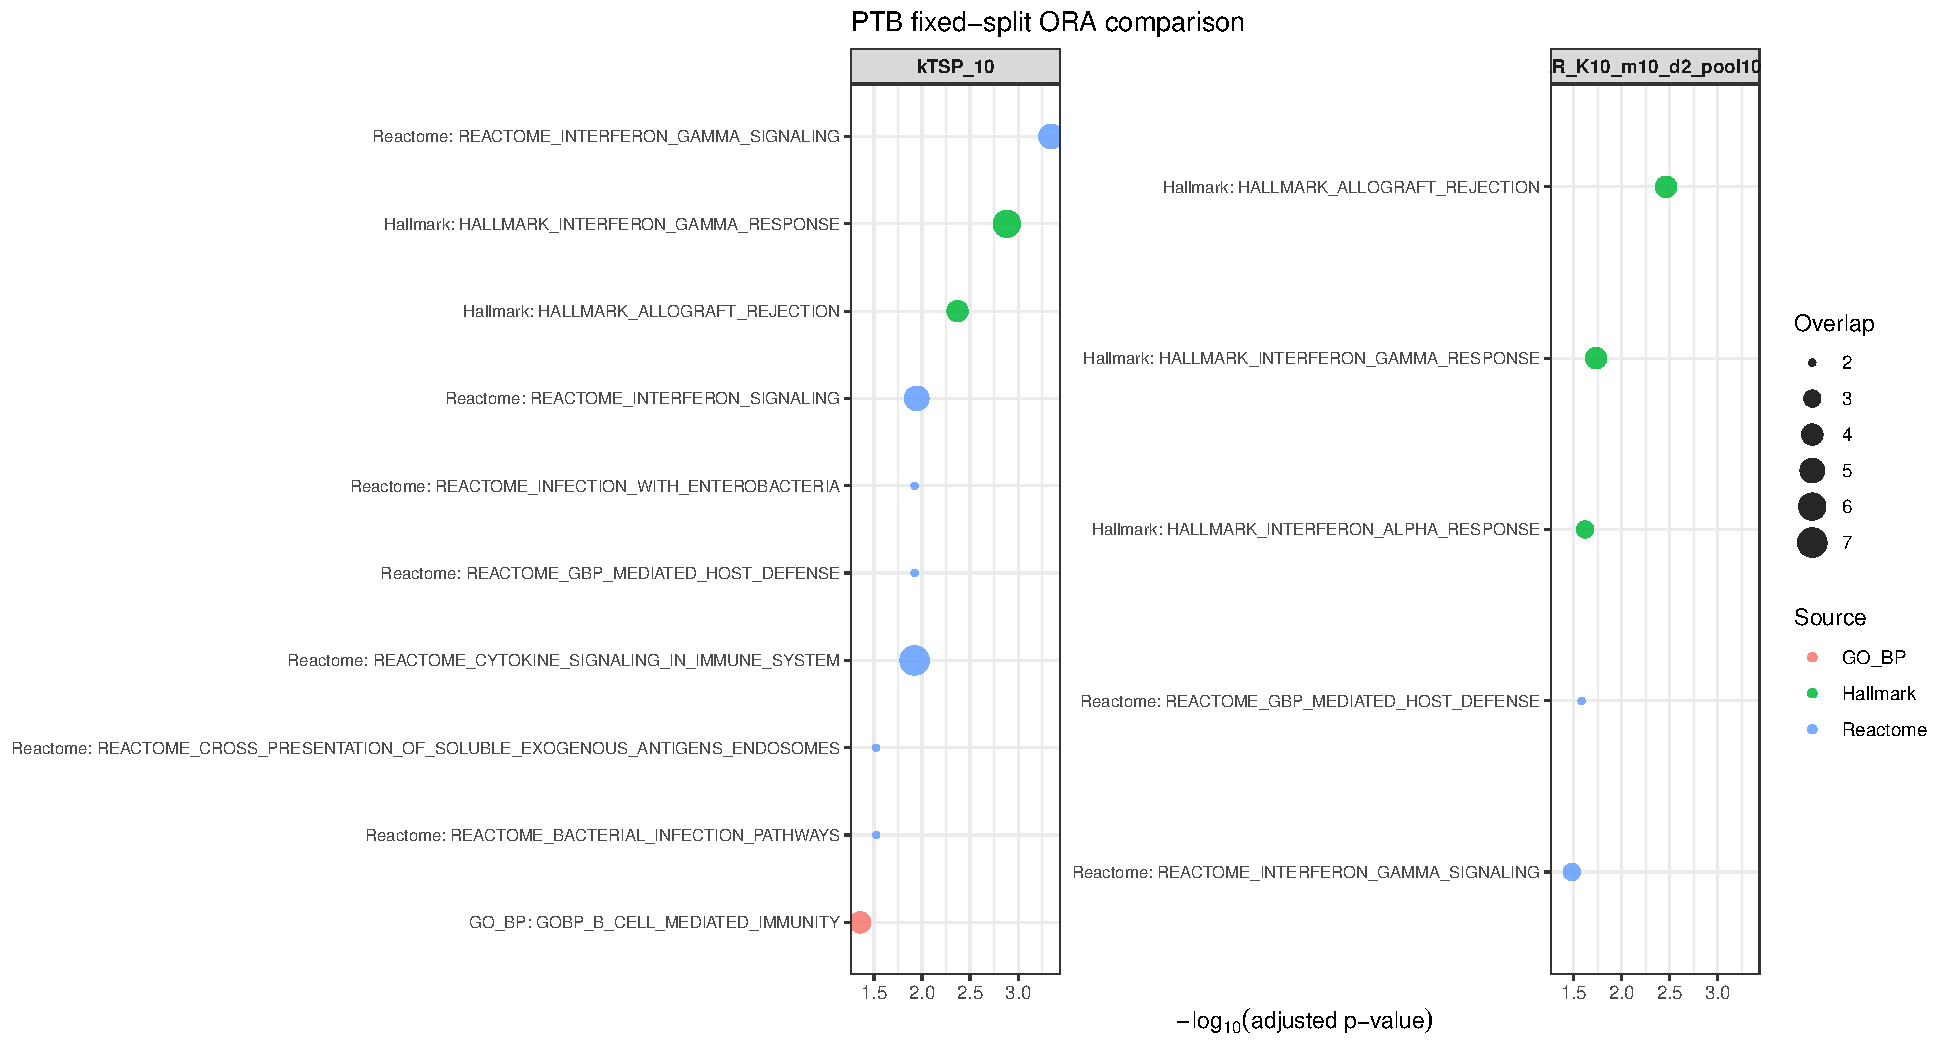
\includegraphics[width=\textwidth]{supp_fig_ptb_fixed_ora_k10.pdf}
\caption{Compact functional-enrichment comparison for the corrected PTB fixed-split ORA. The analysis used the 2000-gene training-only MAD-prefiltered universe reconstructed from the 103-sample training split. The $k$-TSP-10 shortlist yielded 12 FDR-significant terms, whereas the smaller RLR-10 active set yielded 5. Both lists retained immune/host-response and interferon-related enrichment. Point size indicates overlap size and the horizontal axis shows $-\log_{10}(\mathrm{adjusted}\ p\mathrm{-value})$.}
\label{fig:ptb_ora_k10_supp}
\end{figure*}




%%%%
\section{Descriptive support from PTB LOCO}

The \emph{PTB LOCO} setting, based on pulmonary tuberculosis blood transcriptomic cohorts, was included as a descriptive stress test under stronger cohort heterogeneity and was not used as a primary inferential benchmark. At the world level, the same broad qualitative pattern observed in the main benchmark was visible here: the clearest difference between RLR and the corresponding hard-voting configurations appeared in logloss, whereas differences in AUC and F1 were more mixed and depended on configuration.

For the final main-text configurations, the world-level results were as follows.
RLR-10 achieved AUC $=0.962$, F1 $=0.886$, and logloss $=0.245$; RLR-20 achieved AUC $=0.957$, F1 $=0.909$, and logloss $=0.254$; and RLR-50 achieved AUC $=0.961$, F1 $=0.889$, and logloss $=0.263$. The corresponding hard-voting baselines yielded markedly higher logloss values: 0.730 for $k$-TSP-10, 0.529 for $k$-TSP-20, and 0.539 for $k$-TSP-50. Thus, under leave-one-cohort-out evaluation, the clearest difference between the complete RLR pipeline and the corresponding hard-voting configurations remained concentrated in probability-oriented performance.

At the same time, the LOCO results do not support a single dominant configuration across all metrics. The best AUC was achieved by RLR-10, the best F1 by RLR-20, and the lowest logloss again by RLR-10. This variability is consistent with the descriptive role of the LOCO analysis: with only four holdout cohorts and substantial between-cohort heterogeneity, the main purpose of this setting is not to establish a definitive transportability ranking, but to assess whether the probability-oriented pattern observed in the main benchmark remains visible under stronger distributional shift. Under cohort-level holdout evaluation, RLR again showed its clearest difference in the quality of predicted scores rather than in universal dominance across all predictive metrics.

%%%%%

\section{Historical benchmark results}

The \emph{legacy8} benchmark is included primarily for historical positioning rather than for primary inference. In contrast to the main \emph{CompCancer} benchmark, it provides mixed evidence for RLR and does not support a broad superiority claim over classical $k$-TSP. Its main value is therefore contextual: it shows where the complete RLR pipeline remains competitive and where the historical hard-voting baselines remain stronger. Because this historical component is used for contextual positioning rather than for formal comparative inference, it should not be interpreted as a controlled benchmark replacing the primary \emph{CompCancer} analysis.

\subsection{World-level historical results}

\begin{table*}[!htbp]
\centering
\caption{World-level results in the \emph{legacy8} benchmark. Unlike the primary \emph{CompCancer} benchmark, this historical benchmark provides mixed evidence for RLR. In the compact comparison, RLR-10 improves logloss relative to $k$-TSP-10, but for the larger configurations classical $k$-TSP remains stronger at the world level. Accordingly, this benchmark is used for historical positioning rather than as a main source of performance evidence.}
\label{tab:legacy_world}
{\stdtablelayout
\begin{tabular}{lccc}
\toprule
\textbf{Model} & \textbf{AUC} & \textbf{F1} & \textbf{Logloss} \\
\midrule
TSP-1      & 0.767 & 0.692 & 7.655 \\
$k$-TSP-10 & 0.844 & 0.709 & 0.831 \\
$k$-TSP-20 & 0.852 & 0.726 & 0.583 \\
$k$-TSP-50 & 0.850 & 0.732 & 0.418 \\
RLR-10     & 0.839 & 0.699 & 0.711 \\
RLR-20     & 0.845 & 0.708 & 0.670 \\
RLR-50     & 0.846 & 0.697 & 0.530 \\
\bottomrule
\end{tabular}
}
\end{table*}

At the world level, the historical benchmark does not reproduce the main \emph{CompCancer} pattern in full. The compact RLR-10 model still improves logloss relative to $k$-TSP-10 (0.711 vs.\ 0.831), but it is slightly worse in AUC and F1. For the larger comparisons, the picture is less favorable to RLR: both RLR-20 and RLR-50 remain competitive, yet this does not translate into a world-level advantage in the main predictive metrics. Thus, the historical benchmark supports a restrained historical interpretation rather than a strong comparative claim.

\subsection{Dataset-level heterogeneity in historical results}

To show where the historical benchmark is heterogeneous rather than uniformly unfavorable, Table~\ref{tab:legacy_dataset_logloss} reports dataset-level logloss comparisons for the selected compact and higher-capacity models.

\begin{table*}[!htbp]
\centering
\caption{Dataset-level \emph{legacy8} logloss results for selected compact and higher-capacity comparisons. Lower values are better. The compact comparison is often favorable to RLR-10, whereas the higher-capacity comparison is more mixed and does not support a simple global ranking.}
\label{tab:legacy_dataset_logloss}
{\stdtablelayout
\begin{tabular}{lcccc}
\toprule
\textbf{Dataset} & \textbf{$k$-TSP-10} & \textbf{RLR-10} & \textbf{$k$-TSP-50} & \textbf{RLR-50} \\
\midrule
adenocarcinoma & 1.052 & 1.075 & 0.499 & 0.612 \\
breast2        & 1.237 & 1.004 & 0.668 & 1.208 \\
cns            & 1.156 & 2.171 & 0.711 & 1.061 \\
colon          & 1.829 & 0.515 & 0.388 & 0.513 \\
dlbcl          & 0.168 & 0.130 & 0.203 & 0.104 \\
leukemia       & 0.144 & 0.134 & 0.190 & 0.112 \\
ovarian        & 0.606 & 0.381 & 0.388 & 0.341 \\
prostate       & 0.457 & 0.278 & 0.296 & 0.287 \\
\bottomrule
\end{tabular}
}
\end{table*}

The dataset-level view clarifies why the historical benchmark should not be summarized by a single global statement. In the compact comparison, RLR-10 achieves lower logloss on six of the eight datasets (\emph{breast2}, \emph{colon}, \emph{dlbcl}, \emph{leukemia}, \emph{ovarian}, and \emph{prostate}), but performs worse on \emph{adenocarcinoma} and especially on \emph{cns}. In the higher-capacity comparison, RLR-50 improves logloss on four datasets (\emph{dlbcl}, \emph{leukemia}, \emph{ovarian}, and \emph{prostate}) but is worse on the remaining four. Thus, the historical benchmark is genuinely heterogeneous: it contains local successes for RLR, but these are not strong enough to define the overall benchmark-level conclusion.

Overall, the historical benchmark supports only a restrained conclusion. RLR can be positioned meaningfully within the pair-based family and remains competitive on several legacy datasets, especially in the compact regime. However, the strongest empirical support for the method comes from the primary \emph{CompCancer} benchmark and from the PTB structural analyses, not from the historical benchmark.

%%%%%%%%%%%%%%%%%%%%%%%%
\section{Reliability and score-quality diagnostics}

Because the clearest empirical effect of RLR concerns the quality of scores produced from relational evidence, reliability-oriented plots provide useful visual support for the main interpretation of the paper. Figure~\ref{fig:reliability_compcancer} complements the numerical summaries based on logloss, Brier score, and expected calibration error by illustrating how the compared models distribute confidence across prediction bins.

\begin{figure}[!htbp]
\centering
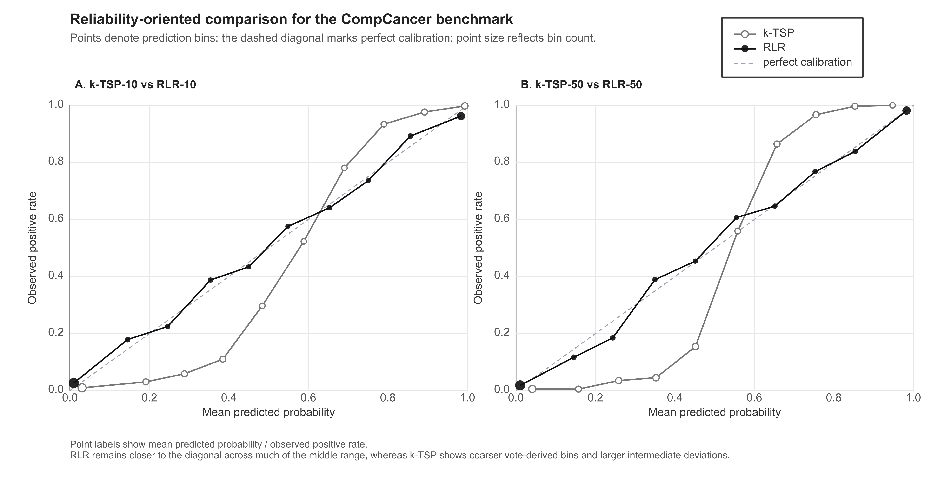
\includegraphics[width=0.95\textwidth]{sup2.pdf}
\caption{Reliability-oriented comparison for the primary benchmark. Each point summarizes one prediction bin, and the dashed diagonal indicates perfect calibration. Across both compact and higher-capacity comparisons, the RLR curves remain closer to the diagonal through much of the intermediate probability range, whereas the classical $k$-TSP baselines concentrate predictions in coarser vote-derived bins and show stronger miscalibration in several middle-confidence regions. The figure therefore complements the numerical logloss, Brier score, and expected calibration error summaries by showing that the main advantage of RLR lies in score behavior rather than in a universal gain in discrimination.}
\label{fig:reliability_compcancer}
\end{figure}

To further characterize the score-quality differences visible in Fig.~\ref{fig:reliability_compcancer}, we additionally examined a pooled Brier-score decomposition for selected compact and higher-capacity comparisons in the \emph{CompCancer} benchmark (Table~\ref{tab:brier_decomposition_compcancer}). These descriptive summaries showed that the lower Brier scores of RLR were associated primarily with a much smaller reliability term, while resolution was also slightly higher for the weighted model in both corresponding nominal-size comparisons. Thus, the probability-oriented advantage of RLR is not reflected only in scalar summary scores such as logloss or ECE, but also in a more favorable reliability--resolution trade-off in pooled out-of-fold predictions.

\begin{table*}[!htbp]
\centering
\caption{Brier-score decomposition for selected models in the pooled \emph{CompCancer} prediction set. Reported values follow the standard reliability--resolution--uncertainty decomposition of the Brier score. These summaries are descriptive and are computed on pooled out-of-fold predictions, so they should not be interpreted as replacements for the dataset-aggregated primary benchmark summaries.}
\label{tab:brier_decomposition_compcancer}
{\stdtablelayout
\begin{tabular}{lccccc}
\toprule
\textbf{Model} & \textbf{Raw Brier} & \textbf{Reliability} & \textbf{Resolution} & \textbf{Uncertainty} & \textbf{Brier from} \\
 & & & & & \textbf{decomposition} \\
\midrule
$k$-TSP-10 & 0.076 & 0.018  & 0.174 & 0.232 & 0.076 \\
RLR-10     & 0.053 & 0.0004 & 0.178 & 0.232 & 0.054 \\
\midrule
$k$-TSP-50 & 0.097 & 0.039  & 0.174 & 0.232 & 0.097 \\
RLR-50     & 0.046 & 0.0002 & 0.186 & 0.232 & 0.046 \\
\bottomrule
\end{tabular}
}
\end{table*}

\section{Approximate runtime characterization in the primary benchmark}

To provide a compact engineering-oriented runtime characterization, we measured approximate wall-clock times on a single representative outer split (\texttt{rep00\_fold00}) for each dataset in the primary \emph{CompCancer} benchmark. These measurements are intended as a practical timing summary rather than as a formal benchmarking study, and should therefore be interpreted descriptively.

For RLR, timings were decomposed into pair ranking, shortlist refinement, train encoding, test encoding, final penalized logistic fitting, and inference. Because the pair-ranking stage is shared across multiple downstream RLR variants on the same split, we report runtime in two complementary ways: (i) a \emph{model-specific} cost that reflects only the downstream cost once the ranked candidate pool is available, and (ii) a \emph{total with shared ranking} cost that attributes the full ranking stage to the model. For classical hard-voting baselines, total train and inference times were measured directly.

Table~\ref{tab:runtime_model_summary} shows that, when the shared ranking stage is fully attributed to each model, RLR is slower than classical $k$-TSP on average. However, most of this difference is due to the pair-ranking stage. Once the ranked pool is already available, the incremental downstream cost of RLR remains small. Table~\ref{tab:runtime_stage_summary} confirms that pair ranking is by far the dominant contributor to RLR runtime, whereas shortlist refinement, encoding, final fitting, and inference are comparatively cheap. Inference itself is fast for both model families.

These timings should not be interpreted as a universal statement about computational superiority, because they were measured on one representative split per dataset and are strongly affected by dataset-specific dimensionality. Their main interpretive value is therefore architectural: in the present pipeline, RLR is computationally dominated by the shared pair-ranking stage, whereas the downstream weighted fitting stages are relatively lightweight.

\begin{table*}[!htbp]
\centering
\caption{Approximate model-level runtime summary in the primary \emph{CompCancer} benchmark. Timings are based on one representative outer split per dataset. For RLR, \emph{model-specific} time denotes the incremental downstream cost once the shared ranked candidate pool is available, whereas \emph{total with shared ranking} attributes the ranking stage to the model.}
\label{tab:runtime_model_summary}
{\stdtablelayout
\begin{tabular}{lcccc}
\toprule
\textbf{Model} & \textbf{Realized} & \textbf{Mean model-specific} & \textbf{Mean total with} & \textbf{Median total with} \\
 & \textbf{$k$ mean} & \textbf{time (s)} & \textbf{shared ranking (s)} & \textbf{shared ranking (s)} \\
\midrule
$k$-TSP-10 & 10.00 & 1.33 & 1.33 & 0.42 \\
RLR-10     & 9.27  & 0.13 & 2.22 & 0.94 \\
\midrule
$k$-TSP-50 & 49.27 & 1.35 & 1.35 & 0.47 \\
RLR-50     & 29.18 & 0.16 & 2.26 & 0.99 \\
\bottomrule
\end{tabular}
}
\end{table*}

\begin{table*}[!htbp]

\centering
\caption{Approximate stage-level runtime summary in the primary \emph{CompCancer} benchmark. For RLR, pair ranking is the dominant stage, whereas shortlist refinement, encoding, final fitting, and inference remain relatively inexpensive. For classical $k$-TSP baselines, training dominates inference.}
\label{tab:runtime_stage_summary}
{\stdtablelayout
\begin{tabular}{lcc}
\toprule
\textbf{Model / stage} & \textbf{Mean time (s)} & \textbf{Median time (s)} \\
\midrule
RLR-10: pair ranking (shared)   & 2.10 & 0.86 \\
RLR-10: shortlist refinement    & 0.01 & 0.00 \\
RLR-10: encoding train          & 0.03 & 0.03 \\
RLR-10: encoding test           & 0.02 & 0.02 \\
RLR-10: final fit               & 0.05 & 0.06 \\
RLR-10: inference               & 0.01 & 0.00 \\
\midrule
RLR-50: pair ranking (shared)   & 2.10 & 0.86 \\
RLR-50: shortlist refinement    & 0.03 & 0.03 \\
RLR-50: encoding train          & 0.04 & 0.02 \\
RLR-50: encoding test           & 0.02 & 0.02 \\
RLR-50: final fit               & 0.07 & 0.06 \\
RLR-50: inference               & 0.01 & 0.00 \\
\midrule
$k$-TSP-10: train               & 1.30 & 0.40 \\
$k$-TSP-10: inference           & 0.02 & 0.02 \\
$k$-TSP-50: train               & 1.33 & 0.44 \\
$k$-TSP-50: inference           & 0.02 & 0.02 \\
\bottomrule
\end{tabular}
}
\end{table*}

Two practical conclusions follow from these measurements. First, the main computational burden of RLR lies in the ranked candidate-pool construction rather than in the downstream weighted fitting stages. Second, once that shared ranking stage is available, the incremental cost of fitting additional RLR variants remains small. 

This distinction is important when interpreting the computational burden of the method: the cost of evaluating a single standalone RLR model is different from the cost of evaluating several related RLR variants on the same ranked pool. Dataset-specific variation was substantial, with the largest observed shared pair-ranking time reaching 11.64~s and the largest observed $k$-TSP training time reaching 8.96~s on the representative split.

\section{Reproducibility note}

The core results reported in the main manuscript were generated from the frozen reference exports corresponding to the four evaluation settings used in the study: the primary \emph{CompCancer} benchmark, the PTB fixed-split case study, the PTB leave-one-cohort-out evaluation, and the historical eight-dataset benchmark. Supplementary exploratory analyses, including the candidate-pool and rank-margin screens, were generated separately and are explicitly identified as sensitivity analyses rather than as additional frozen primary-benchmark estimates.

Across all settings, pair ranking, shortlist construction, hyperparameter selection, and final model fitting were performed strictly within the corresponding training portion of each split or holdout. For RLR, the elastic-net mixing parameter was fixed at $\alpha=0.5$, and the overall regularization strength $\lambda$ was selected with \texttt{cv.glmnet} by internal cross-validation minimizing binomial deviance and using \texttt{lambda.min}. The internal fold count was at most five, reduced when required by the minority-class size, with a minimum of two folds. RLR class labels used for F1 were obtained by thresholding the fitted positive-class probability at 0.5. For classical $k$-TSP, F1 was instead calculated from the labels returned directly by \texttt{SWAP.KTSP.Classify}; it was not recomputed by thresholding the vote-derived score used for AUC and probability-oriented metrics.

For classical $k$-TSP, the score used for AUC, logloss, Brier score, and ECE was obtained from \texttt{SWAP.KTSP.Statistics} and mapped to $[0,1]$ as $(s+k_{\mathrm{real}})/(2k_{\mathrm{real}})$, where $s$ is the returned voting statistic and $k_{\mathrm{real}}$ is the realized number of retained pairs. Score orientation was aligned to the positive class using the training data only. Before logloss calculation, scores were clipped to $[10^{-15},1-10^{-15}]$. ECE used 10 equal-width bins over $[0,1]$, omitted empty bins, and weighted the absolute bin-wise calibration difference by the fraction of samples in each non-empty bin.

The final main-text RLR analyses used the canonical rank-margin setting $m=10$ together with the disjoint shortlist construction $d=2$. Additional exploratory \emph{CompCancer} sensitivity runs over the rank-margin parameter are summarized in Table~\ref{tab:m_sensitivity_world}. These runs were used only as sensitivity checks and not to redefine the main analytical framing.

For the post-hoc calibration analysis of vote-derived $k$-TSP scores, calibration was learned strictly within the outer training data of each \emph{CompCancer} split. Specifically, pooled out-of-fold vote-fraction scores from the outer training portion were used to fit either a Platt-scaling or isotonic calibrator, and the learned mapping was then applied only to the corresponding outer test predictions.

For the PTB fixed-split functional-enrichment analysis, the background universe was reconstructed exclusively from the 103-sample training split using the same MAD top-2000 prefilter applied before pair scoring. Official MSigDB 2026.1.Hs symbol GMT files were used for Hallmark, GO Biological Process, and Reactome. The resulting enrichment analysis therefore uses the same training-side feature restriction as the predictive pipeline and does not use the 44-sample fixed test set or the 106-sample GSE83456 cohort to define the background universe.

The runtime summaries reported in this supplementary document were measured on one representative outer split (\texttt{rep00\_fold00}) per \emph{CompCancer} dataset and should therefore be interpreted as descriptive engineering summaries rather than as formal benchmarking results.

For interpretation, it is important to distinguish between four different quantities: the upstream candidate-pool size, the nominal shortlist size, the fitted global active structure after regularization, and the local active evidence per sample after ternary encoding. These quantities are not equivalent and should not be conflated when discussing model complexity or interpretability.

The cleaned publication repository containing the RLR implementation, frozen experiment configurations, split definitions, analysis scripts, reproducibility documentation, checksums, and selected reference outputs is available in the \href{https://github.com/mczajkowskipb/relative-logistic-regression}{public GitHub repository}. The historical legacy8 processed inputs are documented with checksums and an explicit provenance limitation rather than being represented as newly redistributable source data.

\section*{Concluding supplementary note}

Taken together, the supplementary analyses sharpen the central interpretation of the paper in several ways. First, they show that the finalized disjoint-shortlist formulation benefits materially from a sufficiently large upstream candidate pool. Second, they show that middle rank-margin values yield broadly stable results, whereas an excessively large margin degrades probability-oriented performance by suppressing too much local evidence. Third, they show that an exploratory adaptive-$k$ hard-voting baseline does not materially alter the main comparative picture in the primary benchmark. Fourth, they demonstrate in the PTB case study that RLR does not replace the pair-based signal, but reallocates weight within it while reducing the effective fitted and local active structure. Fifth, they show that the historical benchmark should be interpreted mainly as contextual positioning rather than as the main empirical pillar of the study. Finally, they provide descriptive support from reliability-oriented diagnostics and runtime measurements, clarifying both the score-quality behavior and the engineering cost structure of the proposed pipeline. They also show that post-hoc calibration reduces part of the probability-quality gap of classical hard voting without reproducing the intermediate and larger RLR results, and that the reduced PTB RLR active sets remain compatible with the same broad host-response and interferon-related biological theme.

Overall, these supplementary results reinforce the same restrained conclusion as the main paper: Relative Logistic Regression is best understood as an integrated probabilistic refinement of classical pair-based classification, with its clearest empirical advantage observed in probability-oriented score quality rather than in universal improvement across predictive criteria.

\end{document}
